% tree-s-f-a.tex

% !TEX program = pdflatex
\documentclass[tikz]{standalone}
\usepackage{tikz-qtree}
\newcommand{\red}[1]{\textcolor{red}{#1}}

\begin{document}
  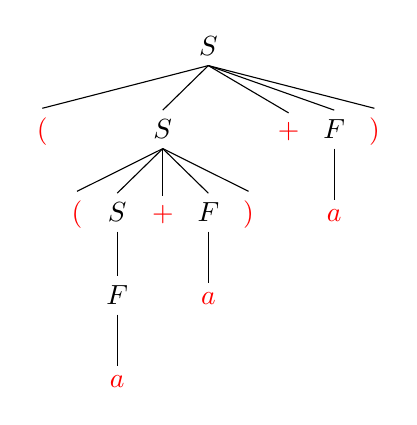
\begin{tikzpicture}
    \Tree [.$S$ [.\red{(} ]
              [.$S$ [.\red{(} ]
                  [.$S$ [.$F$ \red{$a$} ] ]
                  [.\red{+} ]
                  [.$F$ \red{$a$} ]
                  [.\red{)} ]]
              [.\red{+} ]
              [.$F$ \red{$a$} ]
              [.\red{)} ]]
  \end{tikzpicture}
\end{document}